% --------------------------------------------------------------------------
% Template for DCASE 2016 paper; to be used with:
%          dcase2016.sty  - DCASE 2016 LaTeX style file, and
%          IEEEbib.bst - IEEE bibliography style file.
% Adapted from spconf.sty and waspaa15.sty
% --------------------------------------------------------------------------

\documentclass{article}
\usepackage{dcase2016,amsmath,graphicx,url,times,color}
%\usepackage{dcase2016,amssymb,amsmath,graphicx,times,url}

% Example definitions.
% --------------------
\def\defeqn{\stackrel{\triangle}{=}}
\newcommand{\symvec}[1]{{\mbox{\boldmath $#1$}}}
\newcommand{\symmat}[1]{{\mbox{\boldmath $#1$}}}

\newcommand{\ml}[1]{\textcolor{blue}{ Mathieu : #1}}

% Title.
% --------------------
\title{Estimating traffic noise levels using acoustic monitoring \\ a preliminary study}

% Two addresses
% --------------------
\twoauthors
  {Jean-R\'emy Gloaguen, Arnaud Can}
    {Ifsttar - LAE\\
	Route de Bouaye - CS4\\
     Bouguenais, 44344 , FR \\
     jean-remy.gloaguen@ifsttar.fr}
  {Mathieu Lagrange, Jean-Fran\c cois Petiot}
    {Irccyn, UMR CNRS 6597 \\
    \'Ecole Centrale de Nantes\\
	1 rue de la Noe\\
     Nantes, 44321, FR \\
     }

\begin{document}
\ninept
\maketitle

\begin{sloppy}

\begin{abstract}
In this paper, the Non-negative Matrix Factorization is applied for isolating the contribution of road traffic from acoustic measurements in urban sound mixtures. This method is tested on simulated scenes to enable a better control of the presence of different sound sources. The presented first results show the potential of the method.
\end{abstract}

\begin{keywords}
Non-negative Matrix Factorization, road traffic noise mapping, urban measurements
\end{keywords}

\section{INTRODUCTION}
\label{sec:motivations}

Noise in cities is one of the main sources of annoyance essentially caused by road, air an rail traffic. To know better the noise spatial distribution, the number of people impacted and to preserve quiet areas, the European Directive 2002/49/EC \cite{directive} requires that cities over 250 000 inhabitants produce noise maps for road, air and rail traffic. Road traffic noise maps are produced based on a census of the traffic volumes and mean speeds along the main roads which allows estimating their acoustic emission. Assuming knowledge of the city topography, the acoustic propagation within the streets is then calculated. In addition, noise observatories are being deployed in some agglomerations. They aim to facilitate both the mandatory five year update of maps and the validation of the simulated noise maps. Combining classical noise maps with measures would alos be a promising approach to go towards more accurate noise maps \cite{Can} \cite{deCoensel}.


However, to achieve those important goals, we have to isolate the road traffic contribution from measurements  of the sound mixture that contain many others sources. This task is made difficult by the large variety of the sounds that compose the urban sound environments both in terms of spectral properties and temporal structure (car, klaxon, bird, music, horn, siren...) and by the fact that these sounds overlap with each others. Different techniques exists and were shown relevant for recognition or detection in urban environment \cite{Aucouturier} \cite{defreville} but they do not take into account the overlap between the sources. Methods for source separation, such as Computational Auditory Scene Analysis \cite{brown} or Independent Component Analysis \cite{comon} are efficient but are, to the best of our understanding, not suitable for urban applications. Indeed, the first one has been primarily developed to simulate the human auditory system whereas the second one requires as many sensors as sound sources, which is unrealistic in a urban context.

The Non-negative Matrix Factorization (NMF) \cite{lee1999} has the advantage to deal with the overlap between the sound sources. It has been used for many applications in audio domain such as polyphonic music transcription \cite{smaragdis2003} or for source separation of musical content \cite{Virtanen2005}. Thus the NMF seems to be a suitable method for the isolation of the contribution of road traffic from measurements. We propose to apply an NMF scheme on a corpus of urban sound mixtures to validate its ability to estimate the noise level of road traffic. The specificity of urban sound environments, and the fact that the method has, to the best of our knowledge, never been used in this setting, stands as a challenge and requires specific adaptations.

In this paper, we present the implementation of our experimental plan and some first results. Section~\ref{sec:method} exposes the structure of the proposed system based on the NMF framework. Then the experimental protocol is presented in Section~\ref{sec:experiment} and preliminary results are discussed in section~\ref{sec:results}.


\section{Proposed Approach}\label{sec:method}

\begin{figure*}[!ht]
\centering
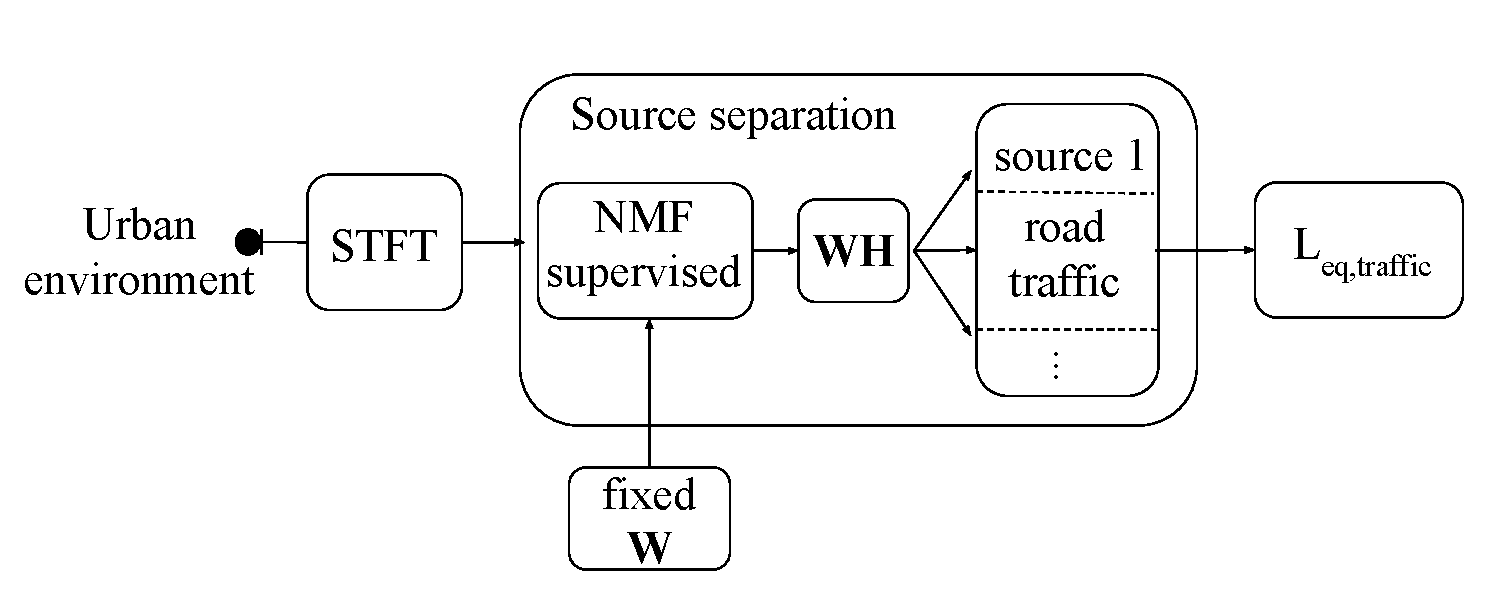
\includegraphics[width=.7\textwidth]{images/bloc1.pdf}
\caption{Block diagram of the proposed method \label{block}}
\end{figure*}

The aim of the system is estimate the level of some predefined sources in the mixture coming from measurements of the urban scene. As can be seen on Figure \ref{block}, the signal is first mapped to a time/frequency plane using the Short Time Fourier Transform. Using the NMF framework, the contribution of the road traffic is isolated and its level is estimated.

\subsection{Non-Negative Matrix Factorization}
The Non-negative Matrix Factorization is a dimension-reduction technique expressed by

\begin{equation}\label{eq:NMF}
\mathbf{V} \approx \mathbf{\tilde{V}} = \mathbf{WH}
\end{equation}

where $\mathbf{V}_{F \times N}$, is the power spectrogram of an audio, $\mathbf{\tilde{V}}$ is the approximate power spectrogram determined by the NMF, $\mathbf{W}_{F \times K}$, is the basis matrix (called dictionary), in our case, representing a set of sound spectra usually found in urban areas. $\mathbf{H}_{K \times N}$ is the feature matrix standing for the temporal variation of each spectrum. All these elements are constrained to be positive leading to additive combinations only. The approximation (\ref{eq:NMF}) is determined by a minimization problem

\begin{equation}\label{eq:minCost}
\underset{\mathbf{W},\mathbf{H} \geq 0}{\text{min }} D(\mathbf{V}\vert\vert \mathbf{WH}).
\end{equation}

$D(\mathbf{V}\vert\vert \mathbf{WH})$ is called function cost, a dissimilarity measure usually belonging to the $\beta$-divergence for the NMF. 3 popular expressions are compared in this study namely the Euclidean distance ($\beta = 2$),

\begin{equation}\label{eq:distEUC}
D_{EUC}(\mathbf{V} \vert \vert \mathbf{WH}) =  \vert\vert \mathbf{V} - \mathbf{WH} \vert\vert , 
\end{equation} 

the Kullback-Leibler divergence, ($\beta = 1$), 

\begin{equation}\label{eq:divKL}
D_{KL}(V\vert\vert WH) = \mathbf{V}\log\frac{\mathbf{V}}{\mathbf{WH}}-\mathbf{V}+\mathbf{WH},
\end{equation}

and the Itakura-Saïto divergence, ($\beta = 0$), 
 
\begin{equation}\label{eq:divIS}
D_{IS}(V\vert\vert WH) = \frac{\mathbf{V}}{\mathbf{WH}} -\log\frac{\mathbf{V}}{\mathbf{WH}}-1.
\end{equation}

Here, the supervised NMF is considered where $\mathbf{W}$ is fixed and only $\mathbf{H}$ is updated iteratively. The choosen algorithm is the maximisation-minimisation algorithm proposed by F\'{e}votte and Idier \cite{fevotte2011}.

\begin{equation}
\mathbf{H} \longleftarrow \mathbf{H}.\left(\frac{\mathbf{W}^T\left[\mathbf{WH}^{\beta-2}.\mathbf{V} \right]}{\mathbf{W}^T \left[ \mathbf{WH} \right]^{\beta-1}}\right)^{\gamma(\beta)}
\end{equation}

where $\gamma(\beta) = 1$ for $\beta \in [1~2]$ and $\gamma(\beta) = \dfrac{1}{2}$ for $\beta = 0$. 

\subsection{Method}

Our approach consists in considering an audio signal recorded in an urban context, sampled at $44,1$ kHz and expressed in the time-frequency domain using a Short Time Fourier Transform. The size of the Hanning window is 5000 points with an overlap of 50 \% and $NFFT = 4096$ points. The temporal resolution chosen is, for the moment, very low ($\Delta t \approx 0,05$ s). 

The supervised NMF is then performed with the spectrogram $\mathbf{V}$ in the input, a fixed dictionary $\mathbf{W}$ and $\mathbf{\tilde{V}}$ in the output. Currently, $\mathbf{H}$ is updated for a number of iteration fixed at 100. When the iteration is over, it is possible to estimate the level of the elements of interest. In the case of road traffic, $\mathbf{\tilde{V}}_{tr} = \left[\mathbf{WH}\right]_{tr}$ which allows to calculate the sound pressure level for each temporal frame

\begin{equation}\label{eq:Lp}
\tilde{L}_{p,n} = 20\log\frac{\sum\mathbf{\mathbf{\tilde{v}}_{\mathbf{n},tr}}}{p_{0}}
\end{equation} 


with $\mathbf{\tilde{v}_{n,tr}}$, the $n$-th frame of matrix $\mathbf{\tilde{V}}_{tr}$ and $ p_{0} = 2\times 10^{-5}$ Pa, the sound pressure of reference. The equivalent traffic sound level estimated, $\tilde{L}_{eq,tr}$, is then determined by

\begin{equation}\label{eq:Leq}
\tilde{L}_{eq,tr} = \frac{1}{T} \sum 10\log \left(10^{\tilde{L}_{p,n}/10}\right)
\end{equation}

where $T$ is the duration of $\mathbf{V}$.\\



\section{EXPERIMENT}\label{sec:experiment}

\begin{figure*}[th!]
\centering
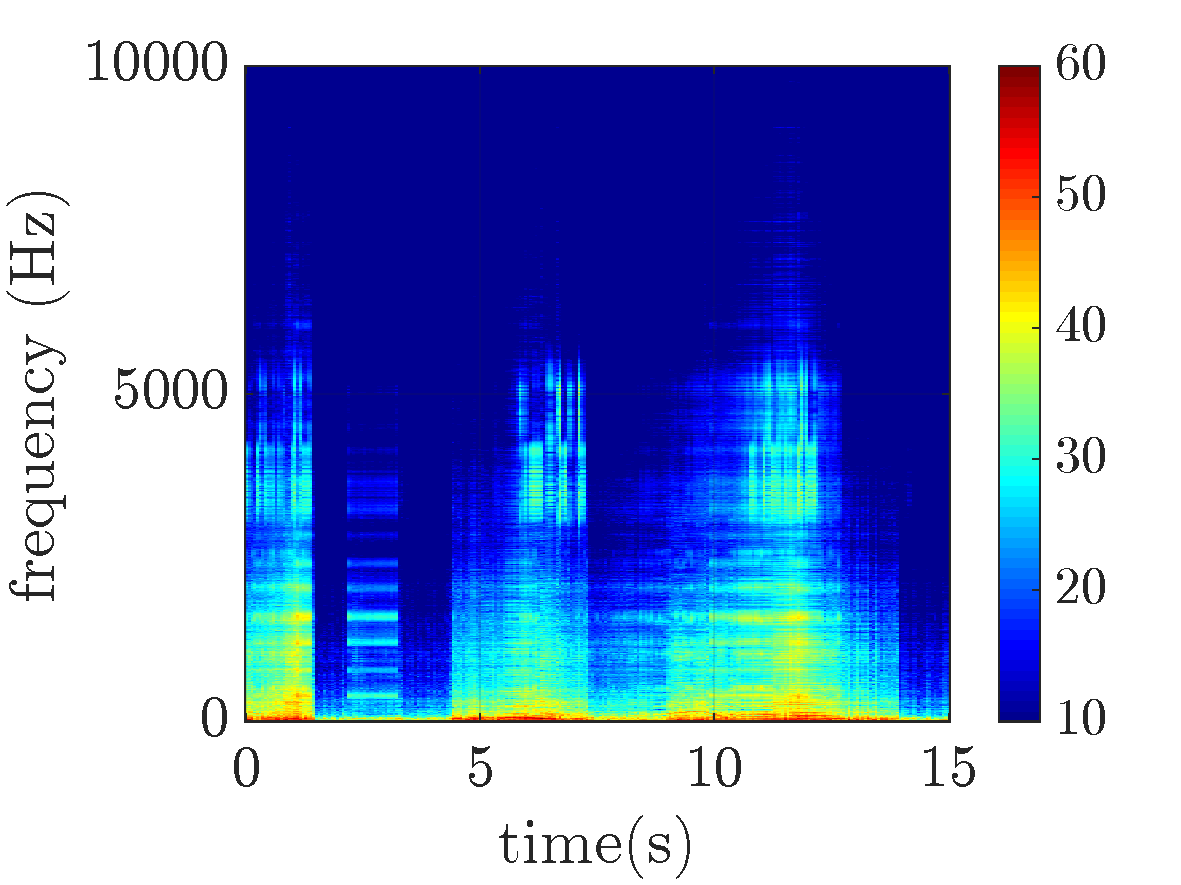
\includegraphics[width=\textwidth]{images/bvak_Sc2_Vapprox_spectre_Euc.pdf}
\caption{Spectrograms of a sound mixture composed with 3 sound classes (\textit{car}, \textit{horn}, \textit{bird}). On the left, the audio given by simScene, on the right, one given by the NMF}
\label{fig:spectrogram}
\end{figure*}

To evaluate the ability of the NMF framework to estimate the road traffic level, we consider simulated sounds mixtures where the actual level of contribution of the traffic is known. This solution ensures controlling the road traffic level, $L_{eq,tr}$, relatively to the other sources in comparison to real recordings where it would not be correctly determined. Furthermore, working on sound mixtures simulated will create a controlled framework where the time of presence of each source is exactly known which allows to produce specific sound environments (animated streets, parks \dots). 

The mixtures are simulated with \textit{simScene} software developed by Mathias Rossignol and Gregoire Lafay \cite{simScene}\footnote{Open-source project available at: \url{https://bitbucket.org/mlagrange/simscene}} which synthesizes sound mixtures from a sound data base of isoled sound events. This tool can control multiple parameters as the event/background ratio, the sample duration, the time between samples \dots Each of these parameters is coupled with a standard deviation to bring some variability between the scenes produced. In the output, an audio file of each sound class is created that allows us to compute the specific contribution of each class present in the scene. The sound data base we use is composed of sound samples provided with the software and completed by others sounds found online\footnote{\url{www.freesound.org}}. The scenes are built with the first half of the data base, the second half being considered as the dictionary $\mathbf{W}$. For tests of feasibility , the first constructed scenes are simple, more realistic scenes fully consistent will be soon produced.\\

For this preliminary study, 20 scenes are created with a duration of 15 s. Each one is composed of 3 classes of sound that can typically be heard in urban areas: \textit{car}, \textit{bird} and \textit{horn}. The aim of this preliminary study is to see the influence of some parameters of the NMF on the quality of the traffic noise levels estimation such as the divergence calculation or the number of iteration. The aim is to perform an NMF on each scene $i$ and to compare $L^i_{eq,tr}$ with $\tilde{L^i}_{eq,tr}$ to evaluate the performance of the method by computing the RMSE

\begin{equation}
RSME = \sqrt{\frac{1}{N}\sum_{i = 1}^N(L^i_{eq,tr}-\tilde{L}^i_{eq,tr})^2}.
\end{equation}

\section{Results}\label{sec:results}

Figure \ref{fig:spectrogram} resumes the spectrograms obtained by simScene (on left) and by the NMF (on right) for one scene with Euclidean distance (\ref{eq:distEUC}) after 100 updates of $\mathbf{H}$. We can observe the bird on the frequency range $\left[3000-6000\right]$ Hz, the horn is characterized by its harmonic content whereas the car is mainly composed of low frequencies with a slower temporal evolution.


From each sound mixture, comparison between $L_{p,t}$ and $\tilde{L}_{p,t}$ for Euclidean distance, Kullback-Leibler and Itakura-Saïto divergences can be made (Figure~\ref{fig:Lp})\\

\begin{figure}[t]
\centering
\centerline{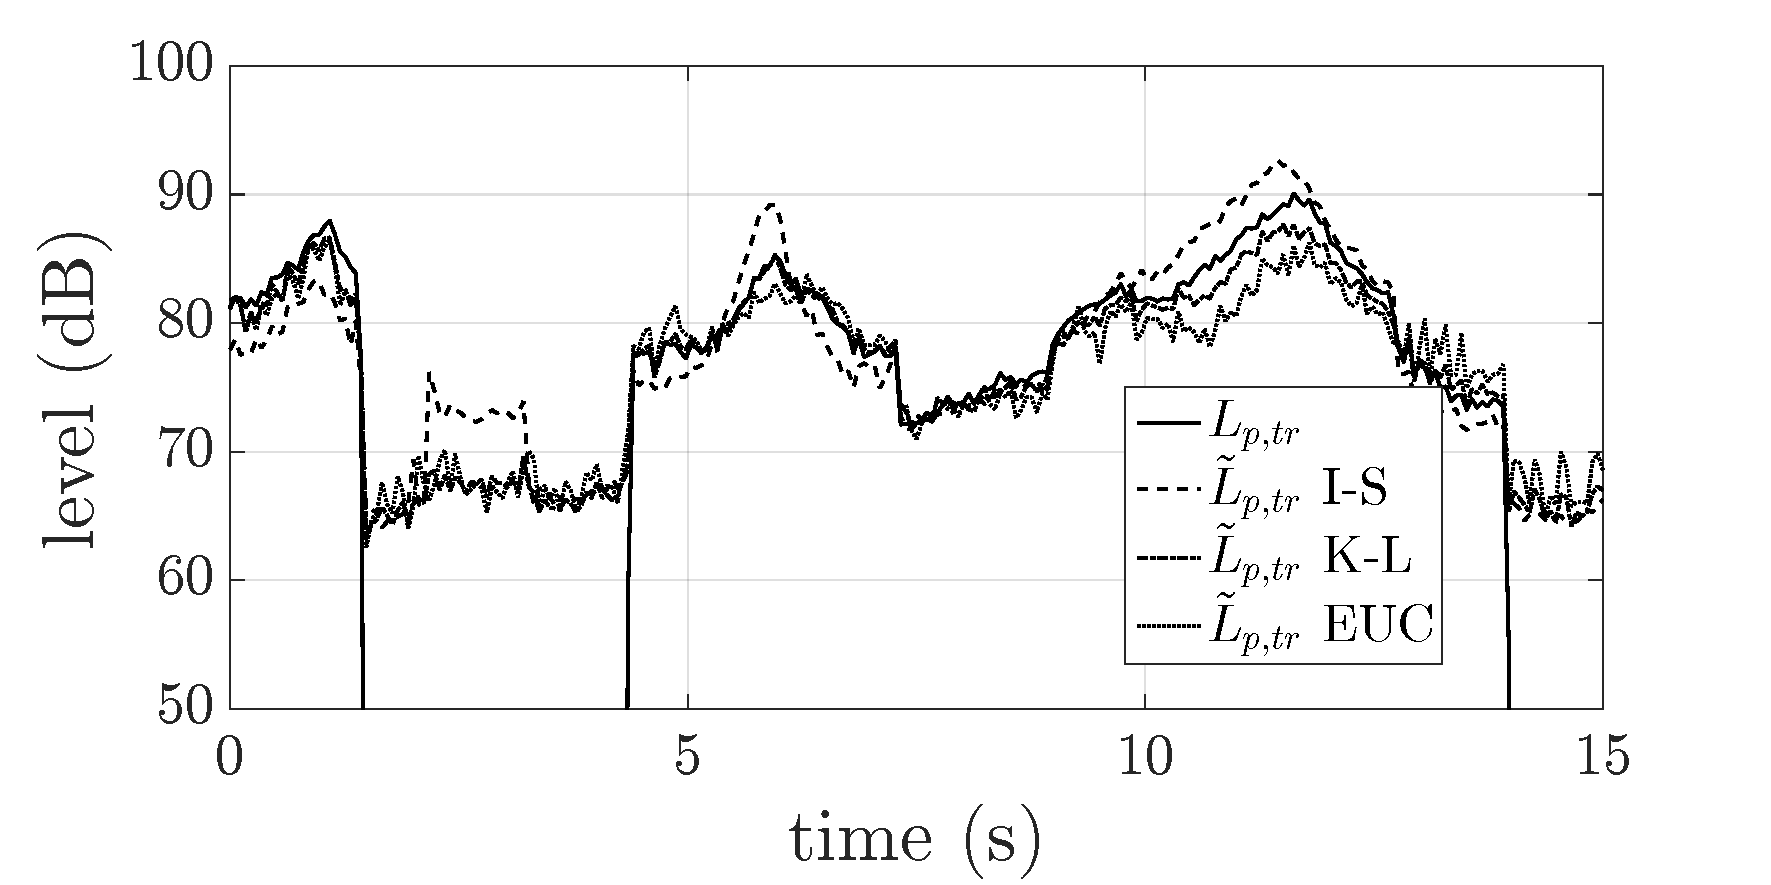
\includegraphics[width=.5\textwidth]{images/Lp_bvak_Sc2_It100_nbCl3.pdf}}
\caption{Sound pressure level estimated and real of one scene for the distance and the two divergences.}
\label{fig:Lp}
\end{figure}

The $L_{p,tr}$ curve corresponds to the sound level of the sound class \textit{car}. For this scene, in the time interval $\left[ 1,5 - 4,5\right] s$, there is no traffic, the sound level is then zero. The sound class \textit{car} describes then the noise background composed of a voice hubbub. Though the noise background sound level is low in comparison with the other class sounds, it thus does not distort the estimations.\\

Let us now consider the RMSE with respect to the number of iterations of the NMF for the three divergences on Figure~\ref{fig:rmse}. The error between $L_{eq,tr}$ and the equivalent sound pressure of the global mixture, $L_{eq}$ is added. This corresponds to the error that would be done if no source separation was done and all the sound sources were taken account without distinction.

\begin{figure}[t]
\centering
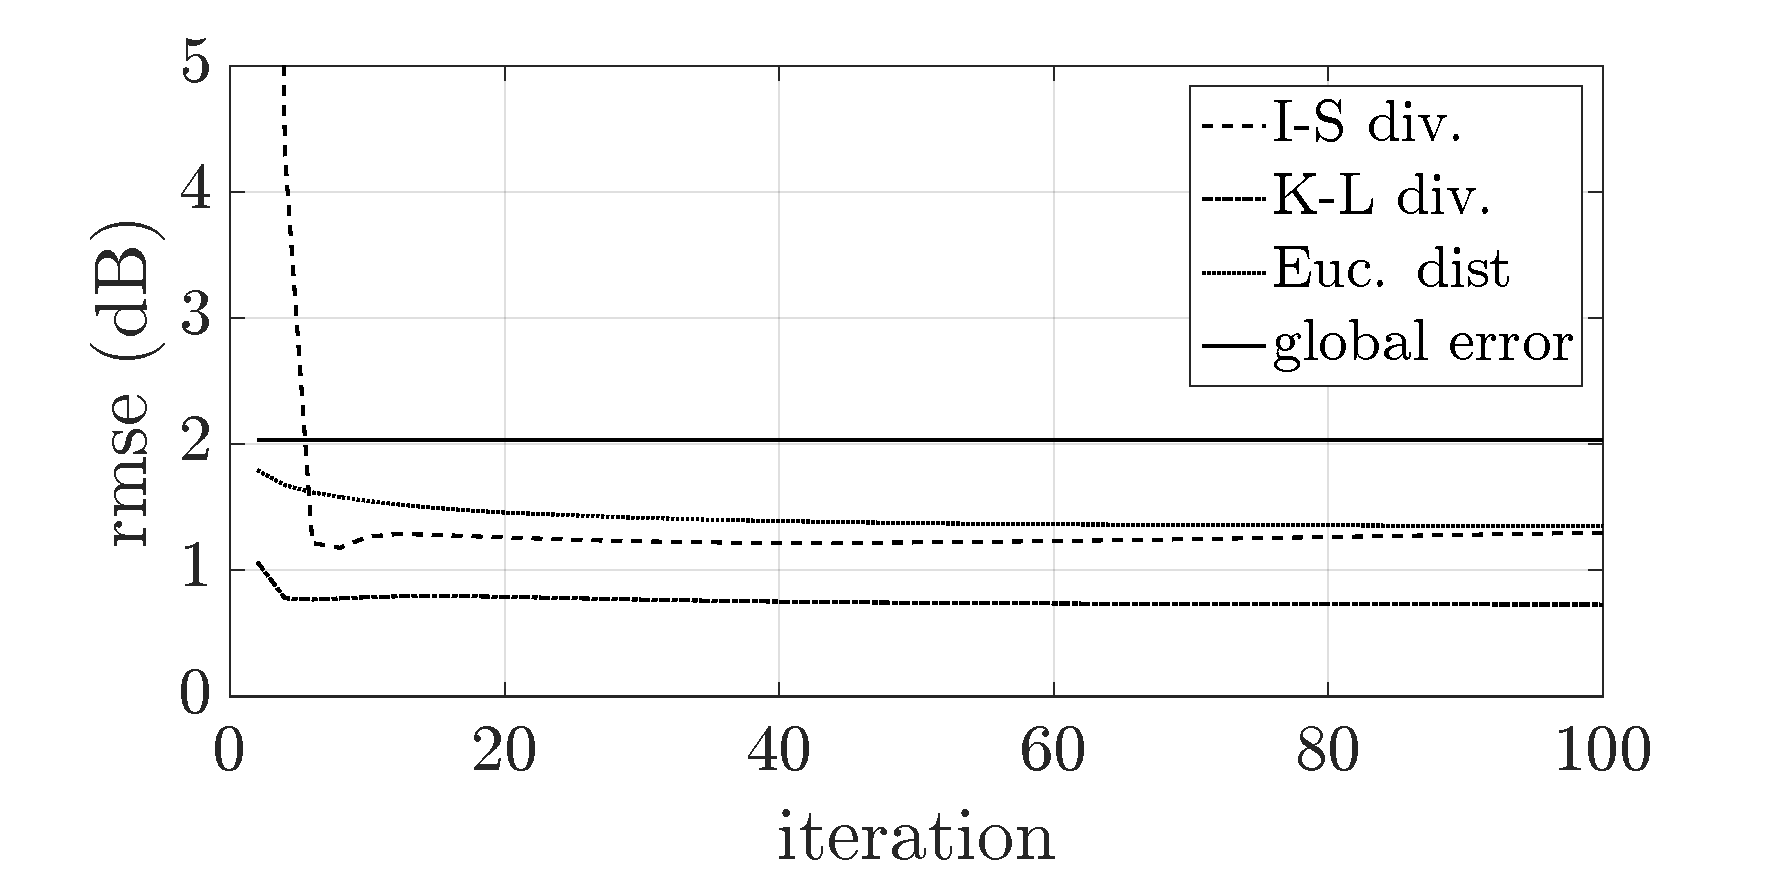
\includegraphics[width=.5\textwidth]{images/comparaison_RMSE_nbCl3.pdf}
\caption{RMSE evolution}
\label{fig:rmse}
\end{figure}

Even if the global error is low ($\approx 2 dB$), the use of the NMF to compute the traffic noise level produce a better estimation than taking the sound mixture with all the sound source. The Kullback-Leibler divergence proposed the most interesting results with the lowest and the most stable RMSE. 
Surprisingly, the Itakura-divergence, despite its scale invariant property \cite{fevotte2011}, has an error similar to the Euclidean distance. This result may change in the future with more complex and more realistic scenes.


\section{Conclusion}

In this article, we proposed to use the supervised NMF framework to estimate the road traffic noise levels based on acoustic measurements achieved in an urban context. In our opinion, such approach would find many applications in the environmental acoustics field such other than improving noise maps with acoustic measurements, for example acoustic biodiversity monitoring. 

%By taking account of the \textit{traffic} element from $\mathbf{W}$ and $\mathbf{V}$, an traffic noise level estimation is obtained.

This method is tested on sound mixtures simulated using the simScene software which allows us to get the exact traffic contribution separately from the other sounds. The method is tested by comparing the equivalent sound level between the traffic element of \textit{simScene} and the estimation given by the NMF for three cost functions. The first results show that this method gives us a better estimation of the sound level than if the source separation is not done, thus demonstrating its interest. Both the road traffic time of presence and amplitude are accurately estimated, advocating for the use of the NMF for isolating the road traffic contribution. The Kullback-Leibler divergence results in the lowest errors will therefore receive specific attention for future work. 

Further investigations with more realist and complex scenes are now required to confirm the behavior of the Kullabck-divergence. Then, some refinements of the NMF including acoustics considerations should improve the goodness of the road traffic noise levels estimation. For instance, the addition of some temporal constraints with a smoothness constraint within the NMF framework such as \cite{fevotteSmooth} \cite{Essid} \cite{virtanenSmooth} to better model the temporal evolution of the traffic elements is currently investigated.


\bibliographystyle{IEEEtran}
\bibliography{refs}

%All manuscripts must be submitted electronically as PDF files. 
%All manuscripts must be formatted for white US letter paper 
%(8.5 $\times$ 11 inches). Please do {\bf not} use A4-size papers. 
%All printed material, including text, illustrations, and charts, 
%must be kept within a print area of 7.0 inches (178 mm) wide 
%by 8.9 inches (226 mm) high. Do not write or print anything outside 
%the print area. The top margin must be 1 inch (25 mm), except for 
%the title page, and the left margin must be 0.75 inch (19 mm).  
%All {\it text} must be in a two-column format. Columns are to be 
%3.29 inches (83.5 mm) wide, with a 0.31 inch (8 mm) space between 
%them. Text must be fully justified. 
%
%
%\section{NUMBER OF PAGES}
%\label{sec:pagelimit}
%
%You are allowed a total of up to 4+1 pages for your DCASE 2016 Challenge 
%and Workshop submissions, with up to 4 pages for technical content including 
%figures and possible references, with the optional 5th page containing only
%references. 
%
%\section{PAGE TITLE SECTION}
%\label{sec:pagestyle}
%
%The paper title (on the first page) should begin 0.98 inches 
%(25 mm) from the top edge of the page, centered, completely 
%capitalized, and in Times 14-point, boldface type.  
%The authors' name(s) and affiliation(s) appear below the title
%in capital and lower case letters.  Papers with multiple authors 
%and affiliations may require two or more lines for this information.
%
%\section{TYPE-STYLE AND FONTS}
%\label{sec:typestyle}
%
%We strongly encourage you to use Times-Roman 
%font. In addition, this will give the proceedings a more uniform 
%look. Use a font that is no smaller than nine point type 
%throughout the paper, including figure captions.
%
%In nine point type font, capital letters are 2 mm high.  
%{\bf If you use the smallest point size, there should be 
%no more than 3.2 lines/cm (8 lines/inch) vertically.}  
%This is a minimum spacing; 2.75 lines/cm (7 lines/inch) 
%will make the paper much more readable. Larger type sizes 
%require correspondingly larger vertical spacing. Please do 
%not double-space your paper. True-Type 1 fonts are preferred.
%
%The first paragraph in each section should not be indented, 
%but all the following paragraphs within the section should 
%be indented as these paragraphs demonstrate.
%
%\section{MAJOR HEADINGS}
%\label{sec:majhead}
%
%Major headings, for example, ``1. Introduction'', should 
%appear in all capital letters, bold face if possible, 
%centered in the column, with one blank line before, 
%and one blank line after. Use a period (``.'') after 
%the heading number, not a colon.
%
%\subsection{Subheadings}
%\label{ssec:subhead}
%
%Subheadings should appear in lower case (initial word 
%capitalized) in boldface. They should start at the left 
%margin on a separate line. 
% 
%\subsubsection{Sub-subheadings}
%\label{sssec:subsubhead}
%
%Sub-subheadings, as in this paragraph, are discouraged. 
%However, if you must use them, they should appear in 
%lower case (initial word capitalized) and start at the 
%left margin on a separate line, with paragraph
%text beginning on the following line. They should be 
%in italics. 
% 
%
%\section{Page Numbering, Header, and Footer}
%\label{sec:page}
%
%Please do {\bf not} paginate your paper. 
%In addition, please do {\bf not} change and remove
%the header and footer.
%
%\section{ILLUSTRATIONS, GRAPHS, AND PHOTOGRAPHS}
%\label{sec:illust}
%
%Illustrations must appear within the designated margins.  
%They may span the two columns. If possible, position 
%illustrations at the top of columns, rather than in 
%the middle or at the bottom. Caption and number every 
%illustration. All halftone illustrations must be clear 
%black and white prints. Colors may be used, but they 
%should be selected so as to be readable when printed 
%on a black-only printer.
%
%Since there are many ways, often incompatible, of 
%including images (e.g., with experimental results) 
%in a \LaTeX\ document, an example of how to do
%this is presented in Fig.~\ref{fig:results}.
%
%% Below is an example of how to insert images. 
%% -------------------------------------------------------------------------
%%\begin{figure}[t]
%%  \centering
%%  \centerline{\includegraphics[width=\columnwidth]{fig1a}}
%%  \caption{Example of a figure with experimental results.}
%%  \label{fig:results}
%%\end{figure}
%
%\section{Equations}
%\label{sec:equations}
%
%Equations should be placed on separate lines and consecutively
%numbered with equation numbers in parentheses flush with the 
%right margin, as illustrated in (\ref{eqn:wave_equation}) 
%that gives the homogeneous acoustic wave equation in
%Cartesian coordinates \cite{eWilliams1999},
%\begin{equation}
%  \label{eqn:wave_equation}
%    \Delta^2p(x,y,z,t)-
%    \displaystyle\frac{1}{c^2}\frac{\partial^2p(x,y,z,t)}{\partial t^2}=0,
%\end{equation}
%where $p(x,y,z,t)$ is an infinitesimal variation of acoustic 
%pressure from its equilibrium value at position $(x,y,z)$ and 
%time $t$, and where $c$ denotes the speed of sound.
%
%Symbols in your equation should be defined before the equation 
%appears or immediately following.  Use (1), not Eq. (1) or 
%equation (1), except at the beginning of a sentence:  
%``Equation (1) is ...''
%
%
%
%\section{FOOTNOTES}
%\label{sec:foot}
%
%Use footnotes sparingly and place them at 
%the bottom of the column on the page on which they are 
%referenced. Use Times 9-point type, single-spaced. To 
%help your readers, avoid using footnotes altogether and
%include necessary peripheral observations in the text 
%(within parentheses, if you prefer, as in this sentence).
%
%\section{REFERENCES}
%\label{sec:ref}
%
%List and number all bibliographical references at the end 
%of the paper. The references should be numbered in order 
%of appearance in the document. When referring to them in 
%the text, type the corresponding reference number in 
%square brackets as shown at the end of this sentence 
%\cite{cJones2003}, \cite{aSmith2000}. For \LaTeX\ users, 
%the use of the Bib\TeX\ style file IEEEtran.bst is 
%recommended, which is included in the \LaTeX\ paper 
%kit available from the DCASE 2016 website \cite{dcase2016web}.
%
%\section{ACKNOWLEDGMENT}
%\label{sec:ack}
%
%The preferred spelling of the word acknowledgment in 
%America is without an ``e'' after the ``g.'' Try to avoid 
%the stilted expression, ``One of us (R. B. G.) thanks ...''
%Instead, try ``R.B.G.\ thanks ...''  Put sponsor 
%acknowledgments in the unnumbered footnote on the first page.

% -------------------------------------------------------------------------
% Either list references using the bibliography style file IEEEtran.bst
%\bibliographystyle{IEEEtran}
%\bibliography{refs}
%
% or list them by yourself
% \begin{thebibliography}{9}
% 
% \bibitem{dcase2016web}
%   \url{http://www.cs.tut.fi/sgn/arg/dcase2016/}.
%
% \bibitem{IEEEPDFSpec}
%   {PDF} specification for {IEEE} {X}plore$^{\textregistered}$,
%   \url{http://www.ieee.org/portal/cms_docs/pubs/confstandards/pdfs/IEEE-PDF-SpecV401.pdf}.
%
% \bibitem{PDFOpenSourceTools}
%   Creating high resolution {PDF} files for book production with 
%   open source tools, 
%   \url{http://www.grassbook.org/neteler/highres_pdf.html}.
%
% \bibitem{eWilliams1999}
% E. Williams, \emph{Fourier Acoustics: Sound Radiation and Nearfield Acoustic
%   Holography}. London, UK: Academic Press, 1999.
% 
% \bibitem{ieeecopyright}
%   \url{http://www.ieee.org/web/publications/rights/copyrightmain.html}.
%
% \bibitem{cJones2003}
% C. Jones, A. Smith, and E. Roberts, ``A sample paper in conference
%   proceedings,'' in \emph{Proc. IEEE ICASSP}, vol. II, 2003, pp. 803--806.
% 
% \bibitem{aSmith2000}
% A. Smith, C. Jones, and E. Roberts, ``A sample paper in journals,'' 
%   \emph{IEEE Trans. Signal Process.}, vol. 62, pp. 291--294, Jan. 2000.
% 
% \end{thebibliography}


\end{sloppy}
\end{document}